\section{Einleitung}

''Ärzte und Zahnärzte haben den Anspruch in Ihren Praxen ein Rufsystem einzusetzen.
Dieses Rufsystem ermöglicht, dass der behandelnde Arzt über einen Knopfdruck Hilfe anfordern oder Behandlungsmaterial bestellen kann.''\cite{aufgabenstellung}
Mit diesem Projekt wurde ein cloudbasiertes Praxisrufsystem realisiert.
Dazu wurde das im Vorgängerprojekt ''IP5 Cloudbasiertes Praxisrufsystem'' umgesetzte Praxisrufsystem erweitert.
Das erweiterte System ermöglicht es Sprachverbindungen zwischen Teilnehmern aufzubauen und Benachrichtigungen zu versenden.
Der Inhalt von empfangenen Benachrichtigung kann automatisch vorgelesen werden.
Als Benutzeroberfläche dient eine native iOS Applikation.
Folgende Abbildungen zeigen die Startseite dieser Applikation (Abbildung 1.1) sowie die Ansicht während eines aktiven Gruppenanrufs (Abbildung 1.2).

\begin{figure}[h]
    \centering
    \begin{minipage}[b]{0.4\textwidth}
        \fbox{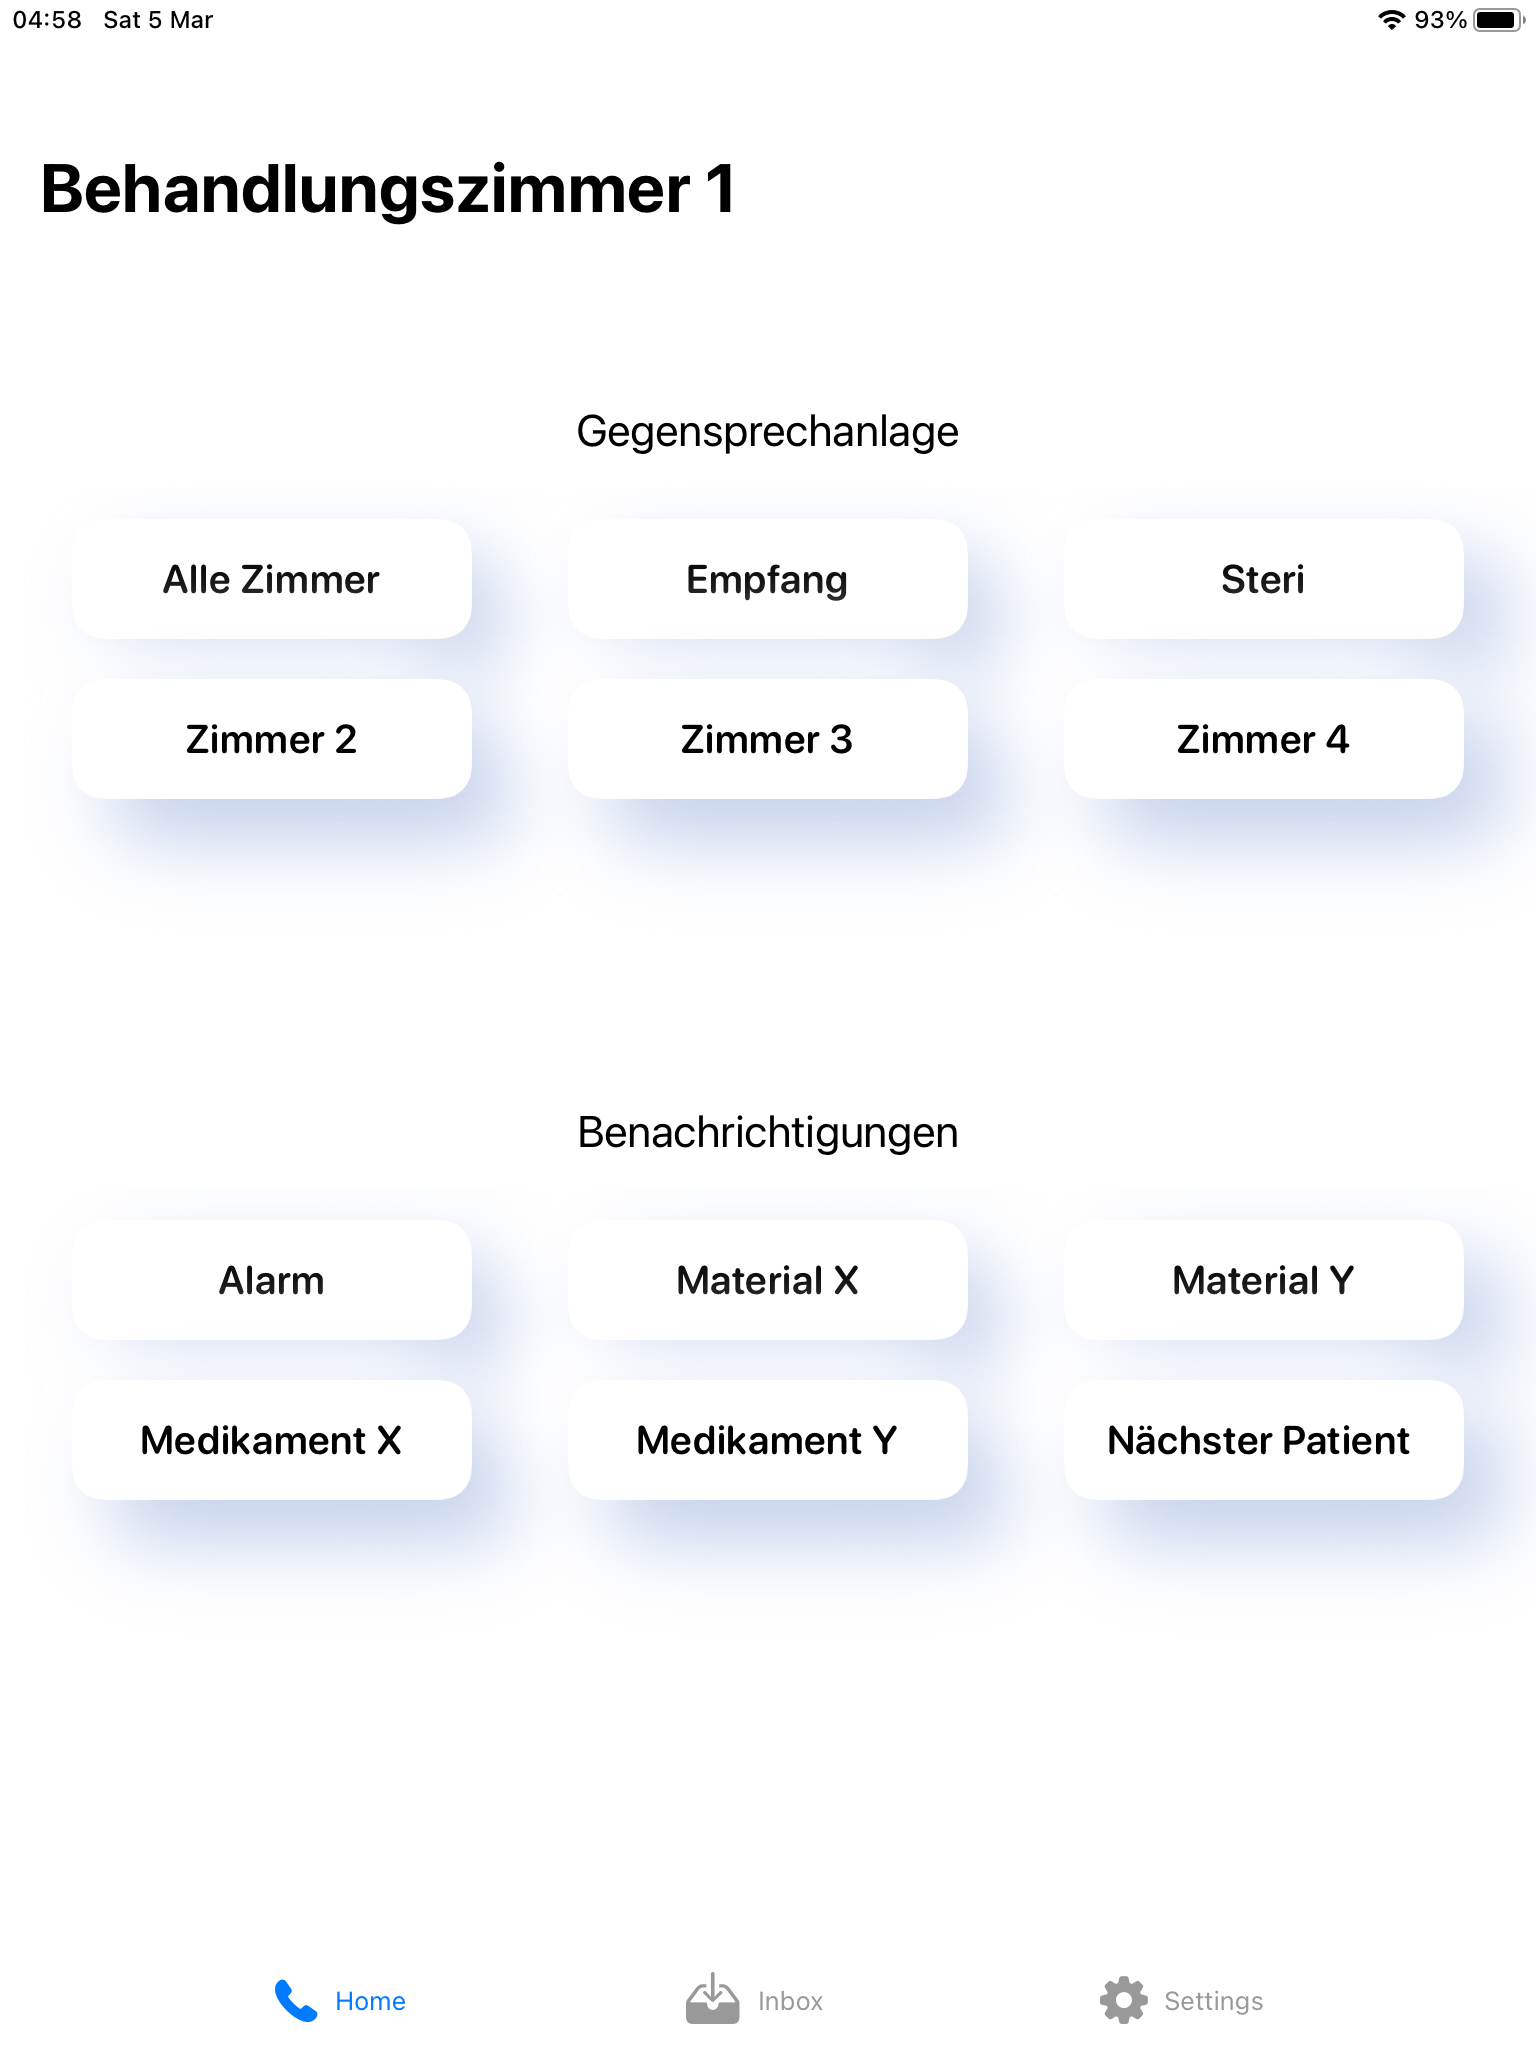
\includegraphics[width=\textwidth]{graphics/screenshots/app/home}}
        \caption{Hauptansicht}
    \end{minipage}
    \hfill
    \begin{minipage}[b]{0.4\textwidth}
        \fbox{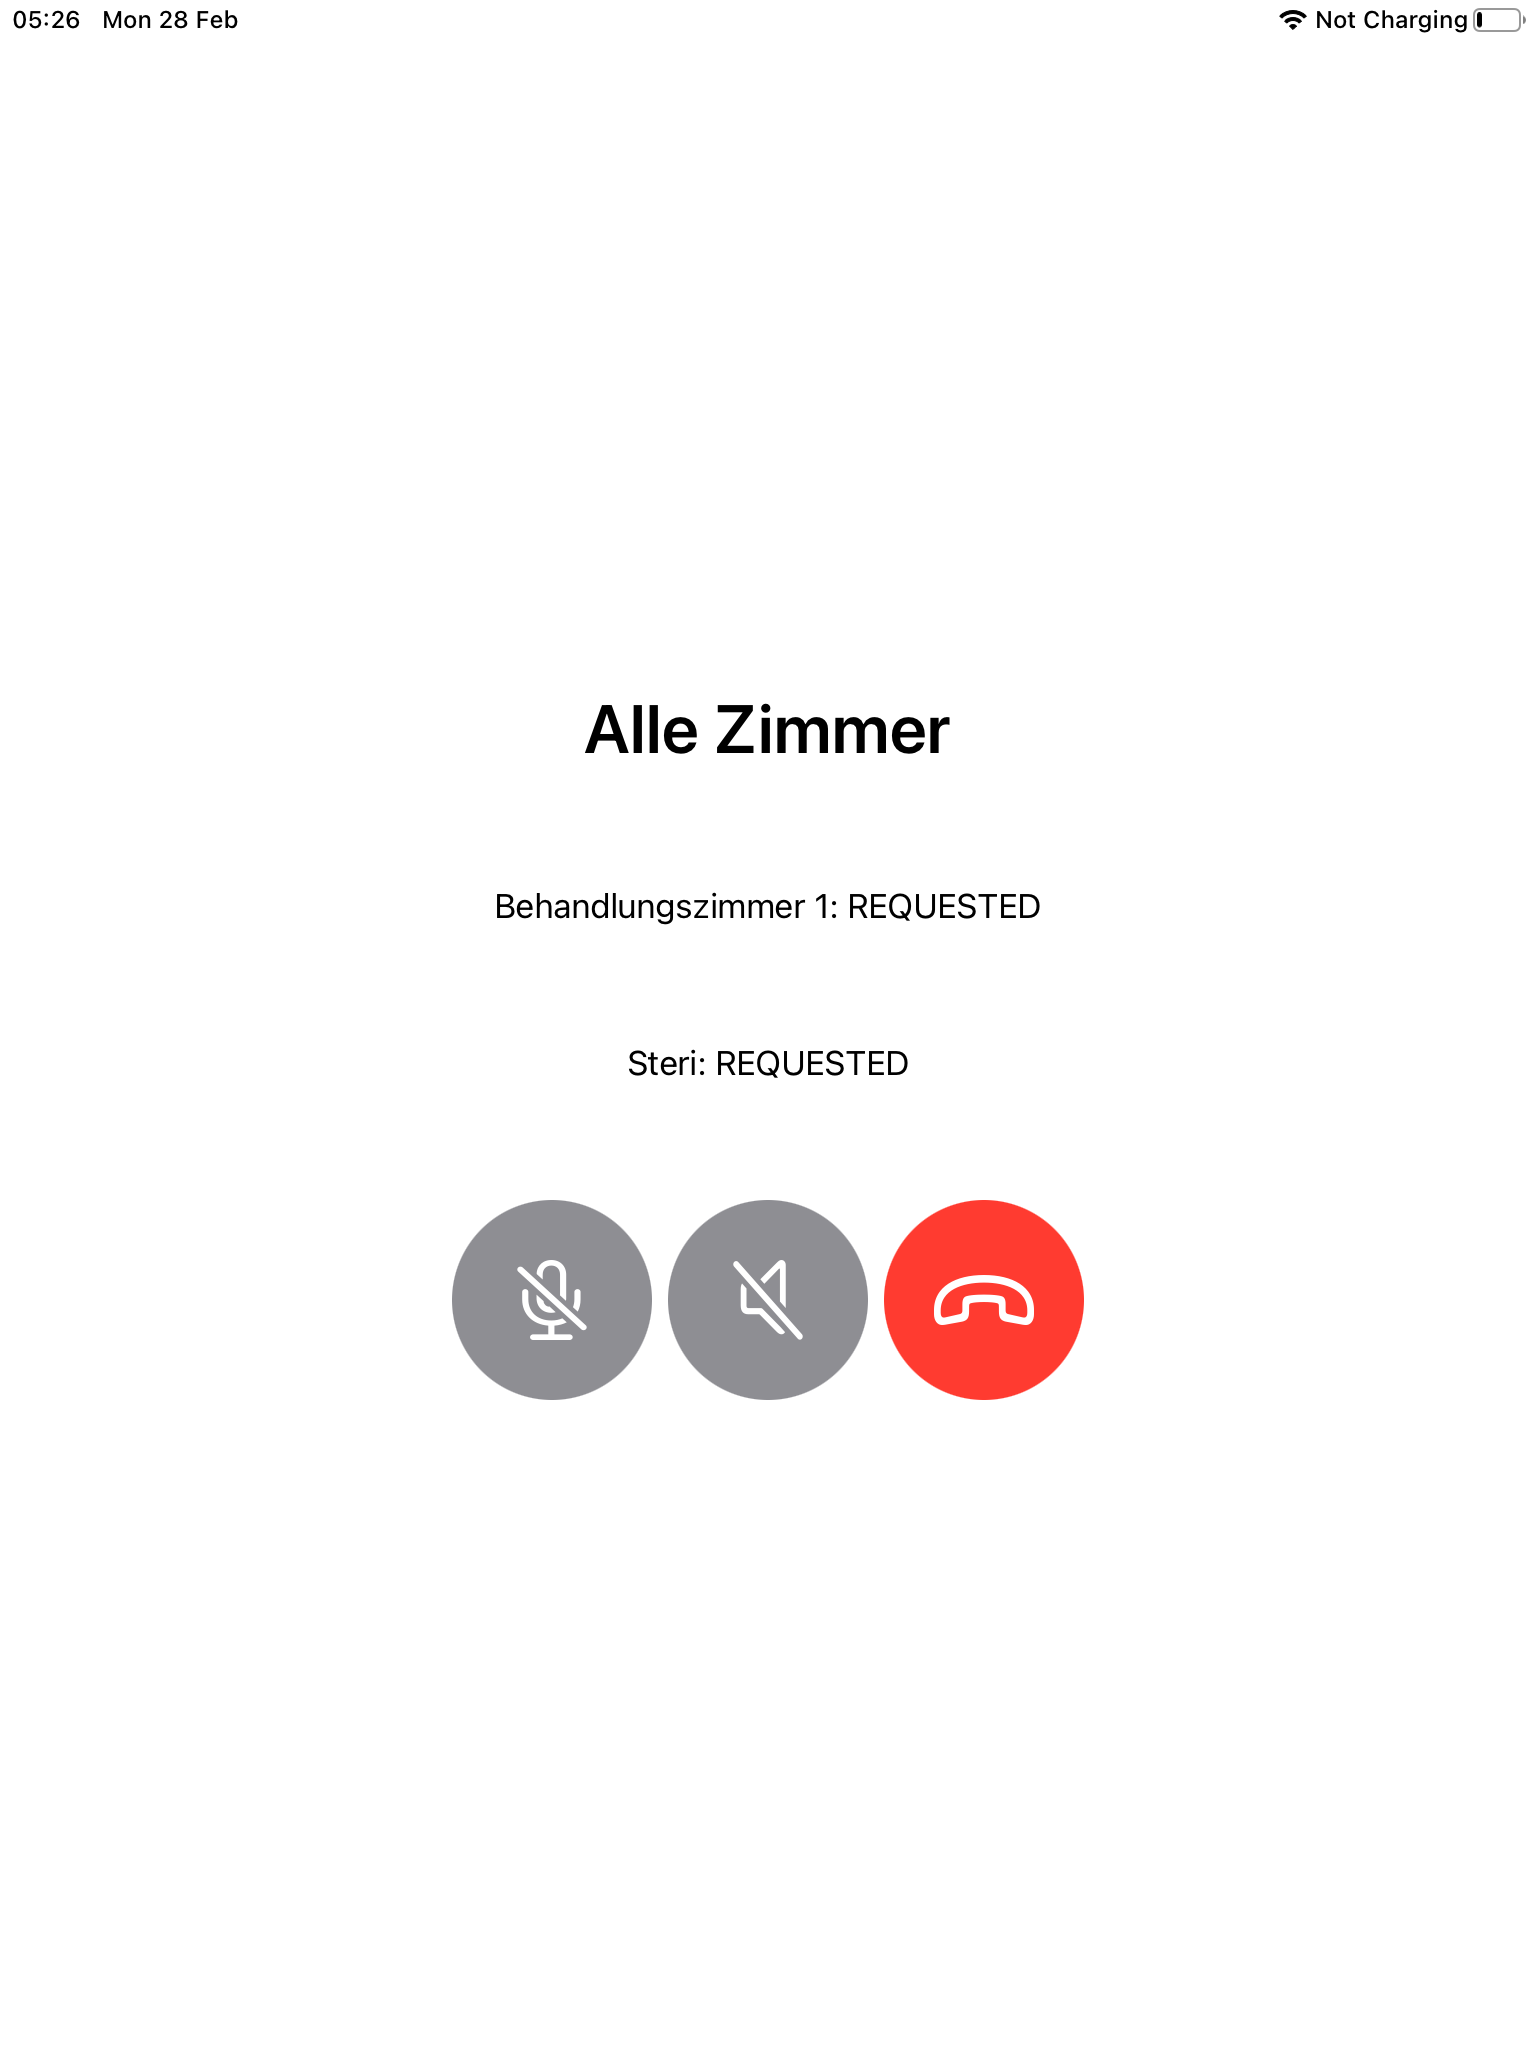
\includegraphics[width=\textwidth]{graphics/screenshots/app/call}}
        \caption{Aktiver Anruf}
    \end{minipage}
    \label{fig:MobileClient-ScreensIntroduction}
\end{figure}

Auf der Startseite der Applikation können per Knopfdruck Benachrichtigungen versendet und Sprachverbindungen gestartet werden.
Empfangene Benachrichtigungen werden als Push-Benachrichtigung angezeigt und in einer Inbox gesammelt.
Bei entsprechender Konfiguration wird zudem der Inhalt empfangener Benachrichtigungen vorgelesen.
Sprachverbindungen können zwischen zwei oder mehr Teilnehmern aufgebaut werden.
Das System unterstützt sowohl private Gespräche als 1:1 Verbindungen wie auch Gruppenunterhaltungen als 1:n Verbindungen.

Welche Buttons und damit welche Benachrichtigungen und Sprachverbindungen zur Verfügung stehen, wird durch Administratoren konfiguriert.
Die Konfiguration von Buttons für Sprachverbindungen beinhaltet, mit welchen Empfängern eine Verbindung aufgebaut wird.
Die Konfiguration von Buttons für Benachrichtigungen definiert den Inhalt der Benachrichtigung, welche Empfänger sie erhalten und ob die Benachrichtigung vorgelesen wird.
Die Verwaltung dieser Konfiguration kann durch eine Weboberfläche vorgenommen werden.
Abbildung 1.3 zeigt die Übersicht verfügbarer Benachrichtigung in dieser Weboberfläche.

\begin{figure}[h]
    \centering
    \begin{minipage}[b]{0.9\textwidth}
        \fbox{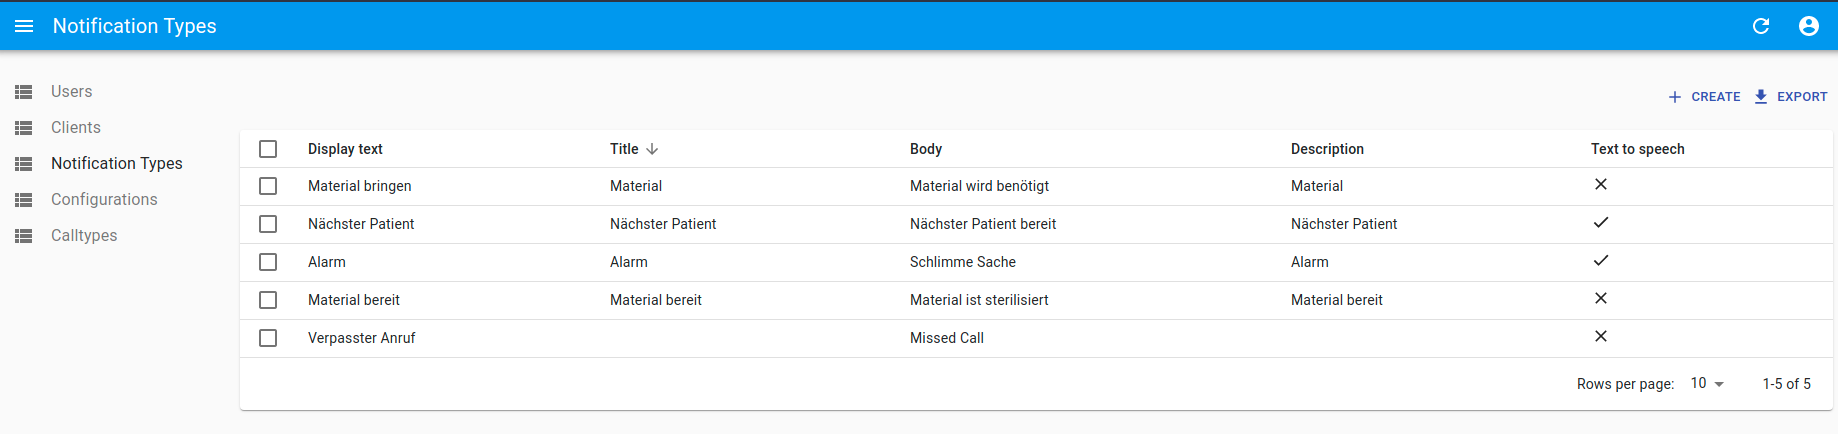
\includegraphics[width=\textwidth]{graphics/screenshots/admin_ui_notification_types}}
        \caption{Praxisruf Startseite}
    \end{minipage}
    \label{fig:AdminUI-Introduction}
\end{figure}

Die Grundlage für das umgesetzte Praxisrufsystem wurde im Rahmen der Projektarbeit ''IP5 Cloudbasiertes Praxisrufsystem'' erarbeitet.
Im Rahmen des Vorgängerprojektes wurde ein Praxisrufsystem mit eingeschränktem Funktionsumfang realisiert.
Die in diesem Projekt entwickelte Lösung ist eine Erweiterung des bestehenden Systems.
Das zuvor umgesetzte System unterstützte das Versenden und Empfangen von Benachrichtigungen.
Sprachsynthese für Benachrichtigungen und Sprachverbindungen für eine Gegensprechanlage konnten im Rahmen des Vorgängerprojektes nicht umgesetzt werden~\cite{ip5}.
Die zentrale Aufgabenstellung für dieses Projekt ist es, das System zu erweitern so, dass Benachrichtigungen vorgelesen und Sprachverbindungen aufgebaut werden können.
Die Bedienung des Praxisrufsystems muss weiterhin über eine mobile Applikation möglich sein.
Dazu soll eine neue, native iOS Applikation entwickelt werden.
Diese ersetzt die bestehende App und muss alle bestehenden Funktionen unterstützten.
Sie muss zudem Sprachverbindungen zu anderen Teilnehmern aufbauen und den Inhalt von Benachrichtigungen vorlesen können.

Wie in der Aufgabenstellung beschrieben, hat eine Marktanalyse im Vorfeld dieses Projektes gezeigt, dass bestehende kommerzielle Praxisrufsysteme vorwiegend veraltete Kommunikationstechnologien einsetzten.
Diese Systeme seien deshalb aufwändig zu installieren und skalieren schlecht.
Sie können weiter nicht einfach in ein TCP/IP-Netzwerk eingebunden oder über externe APIs angesteuert werden~\cite{aufgabenstellung}.
Das im Rahmen des Vorgängerprojektes umgesetzte System löst diese Probleme teilweise.
Mit der Serverkomponente ''Cloudservice'' bietet das System einen zentralen Dienst, welcher über eine Http-Schnittstelle ansprechbar ist.
Diese ermöglicht die Verwaltung der Systemkonfiguration und leitet Benachrichtigung anhand der Konfiguration an relevante Empfänger weiter.
Dadurch ist es einfacher möglich, das System in Netzwerke einzubinden, zu skalieren und neue Endgeräte anzubinden.
Das Vorgängersystem unterstützt aber noch nicht alle Funktionen, die ein Praxisrufsystem bieten muss.
Die meisten kommerziell erhältlichen Lösungen können als Gegensprechanlage verwendet werden~\cite{aufgabenstellung}.
Ein konkurrenzfähiges Praxisrufsystem muss deshalb als Gegensprechanlage verwendet werden können.
Mit der Integration von Sprachsynthese für Benachrichtigungen kann sich das System weiter von bestehenden Lösungen absetzten.
Ein weiterer Schwachpunkt des Vorgängerprojektes ist die darin entwickelte mobile Applikation.
Diese wurde mit einer geteilten Codebasis für iOS und Android entwickelt.
Im Fazit des Vorgängerprojekts wurde festgehalten, dass diese Applikation neu als native Applikation entwickelt werden sollte.
Dadurch könne effizienter Betrieb, Wartung sowie Hardware- und Betriebssystemkomaptibilität langfristig gewährleistet werden~\cite{ip5}.
Deshalb ist auch die Neuentwicklung und Erweiterung der mobile App als native Applikation zentraler Bestandteil der Aufgabenstellung.

Das umgesetzte System besteht aus drei Applikationen.
Der zentrale Cloudservice dient zur Verwaltung der Konfiguration und dem Vermitteln von Nachrichten zwischen Endgeräten.
Das Admin UI bietet eine Weboberfläche, mit der die Konfiguration des Cloudservice verwaltet werden kann.
Mit dem Mobile Client bietet das System neu eine native iOS App über welche Sprachverbindungen aufgebaut und Benachrichtigungen versendet/empfangen werden können.
Für das Versenden von Benachrichtigungen senden Mobile Clients HTTP Anfragen an den Cloudservice.
Der Cloudservice findet in der Konfiguration alle relevanten Empfänger und leitet die Benachrichtigung an diese weiter.
Für die Zustellung von dem Cloudservice an Mobile Clients wird Firebase Cloud Messaging verwendet.

Das Vorlesen von Benachrichtigungen wurde mit einer Anbindung an Amazon Polly im Cloudservice implementiert.
Bei Amazon Polly handelt es sich um einen Dienst zur Sprachsynthese von Amazon Webservices~\cite{aws_polly}.
Der Cloudservice bietet eine Http-Schnittstelle, über welche Clients Sprachdaten für Benachrichtigungen beziehen können.
Durch diese Lösung müssen die Endgeräte die Anbindung an den Provider für Sprachsynthese nicht selbst implementierten.
Dies bietet insbesondere die Vorteile, dass der Provider leicht ausgewechselt werden kann und dass die Anbindung von zukünftigen Plattformen übernommen werden kann.

\begin{figure}[h]
    \centering
    \begin{minipage}[b]{0.6\textwidth}
        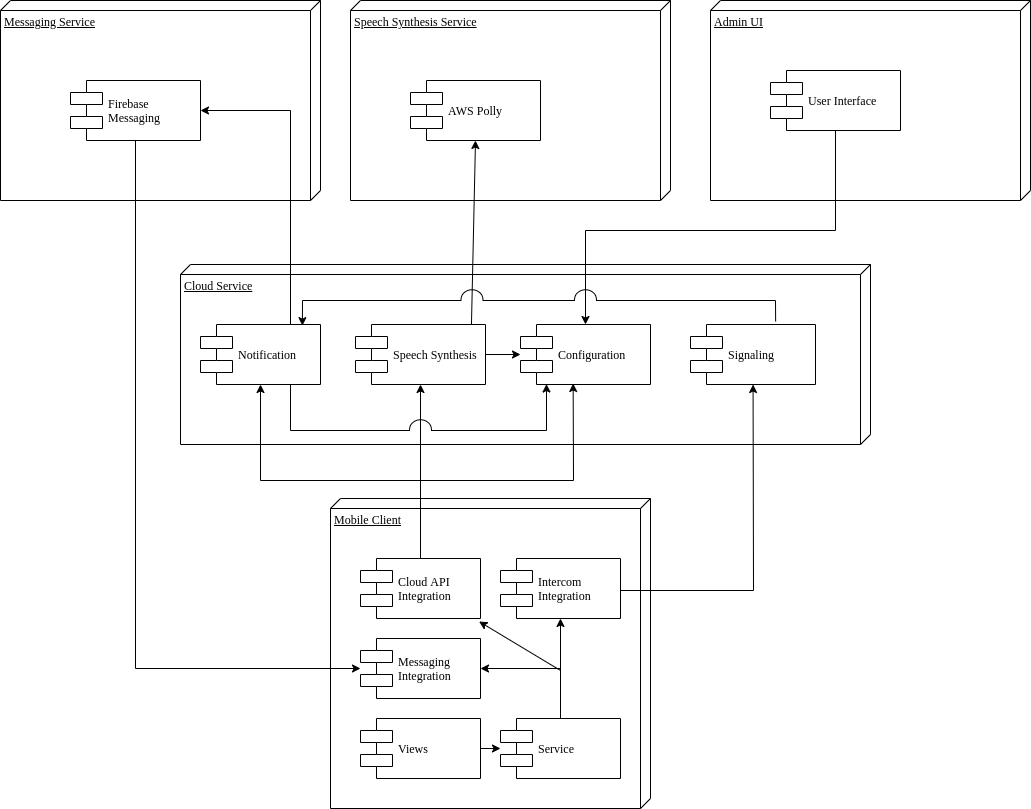
\includegraphics[width=\textwidth]{graphics/diagramms/Component_System_V03}
        \caption{Systemarchitektur Praxisruf}
    \end{minipage}
\end{figure}

Abbildung 1.4 gibt einen Überblick über die Komponenten des umgesetzten Systems.
Dabei sind Module, die im Rahmen dieses Projektes entwickelt oder neu integriert werden, grün umrandet.
Pfeile in der Grafik stellen den Informationsfluss zwischen Komponenten dar.

Sprachverbindungen zwischen Mobile Clients werden als Peer-To-Peer Verbindungen aufgebaut.
Diese Verbindungen wurden mit der Technologie WebRTC umgesetzt.
WebRTC basiert auf einem offenen Standard, welcher Echtzeitkommunikation für mobile Applikationen und Browser Applikationen ermöglicht~\cite{webrtc}.
Damit Peer-To-Peer Verbindungen zwischen Endgeräten aufgebaut werden können, müssen diese Signalmeldungen austauschen können.
Um dies zu ermöglichen, wurde der Cloudservice um ein Modul ''Signaling'' erweitert.
Dieses Modul bietet eine Websocket-Schnittstelle, über welche synchrone Meldungen ausgetauscht werden können.
Jedes Endgerät, das für Sprachverbindungen verfügbar ist, baut bei der Anmeldung im System eine langlebige Verbindung zum Signaling-Modul auf.
Über diese Verbindung sendet und empfängt es alle Signalmeldungen, die für den Verbindungsaufbau notwendig sind.

Im folgenden Bericht werden die erarbeiteten Konzepte und Resultate detailliert beschrieben.
Zunächst werden Vorgehensweise, Projektplan und die Organisation des Projekts vorgestellt.
Anschliessend werden die Anforderungen, welche zu Beginn des Projekts definiert wurden, beschrieben.
Es folgen eine Zusammenfassung der Ausgangslage und eine Technologie Evaluation für Sprachsynthese und Gegensprechanlage.
Dabei werden mögliche Optionen beschrieben und anschliessend begründete Entscheidungen getroffen.
Das darauffolgende Kapitel gibt eine Einführung in die technischen Grundlagen und Protokolle für WebRTC.
Im anschliessenden Hauptteil wird das detaillierte technische Konzept für Funktionsweise und Architektur des Systems dokumentiert.
Es wird beschrieben, wie die Funktionen Gegensprechanlage und Sprachsynthese umgesetzt werden.
Dabei wird insbesondere darauf eingegangen, wie die bestehende und neue Funktionen in einer nativen iOS Applikation integriert werden.
Weiter werden die notwendigen Abläufe, Kommunikationskanäle und Datenmodelle beschrieben.
Nach dem Konzept werden die Resultate zusammengefasst und die umgesetzten Ansichten des nativen iOS App abgebildet.
Am Ende der Arbeit stehen ein Fazit und Schlusswort mit Empfehlungen für das weitere Vorgehen.

\clearpage
